\section{Fundamentos y herramientas\label{FunAndTools}}

En esta sección vamos a realizar una breve introducción al Big Data y haremos un estudio de las herramientas que escogemos para entender mejor por qué se han seleccionado.\par

\subsection{Qué es el Big data\label{WhatIsBigD}}

El motivo por el que se inició este nuevo paradigma “Big Data” fue debido a la gran explosión de datos que tiene lugar con el surgimiento de tecnologías como la Web 2.0, los smartphones e IoT. Se calcula que se emiten más de 30 Terabytes de información cada segundo en el mundo \cite{BD-2} y el IDC predice que desde 2010 a 2020 el volumen de datos aumentará por 50 llegando por encima del Zettabyte de datos \cite{BD-2}. Por tanto, este nuevo paradigma surge debido a que los paradigmas tradicionales no tenían la capacidad de dar una respuesta al manejo de grandes volúmenes de datos.\par

En 2001, Doug Laney describe el Big Data mediante los siguientes términos conocidos como las 3 Vs del Big Data \cite{BD-4}:

\begin{itemize}
\item Volumen: El conjunto de datos debe ser grande.
\item Velocidad: Debe existir una forma rápida de que lleguen los datos, procesarlos y devolverlos.
\item Variedad: Los datos pueden ser de cualquier tipo ya sea alfanumérico, imágenes, sonidos, videos, etc…
\end{itemize}

No obstante, a día de hoy, IBM introdujo la cuarta V del Big Data que se define como Veracidad, es decir, que los datos sean lo más reales posible, ya que cuando manejamos esta cantidad de datos, encontrar datos erróneos se hace más probable. Esto quiere decir que en Big Data nos encontramos el gran reto de gestionar gran cantidad de datos de una forma óptima \cite{BD-5}.\par

Por otra parte, encontramos tres formas de tratar los datos según las diferentes necesidades que aparecen. A la hora de analizar los datos debemos tener en cuenta si se procesarán los datos del pasado, lo que implicaría reportes analíticos, entre otras aplicaciones; si se procesan en tiempo real, lo que quiere decir que se debe mostrar lo que pasa en el momento, y si queremos saber lo que pasará en el futuro, lo que implica procesos de machine learning entre otros \cite{BD-3}.\par

Por otro lado, encontramos un cambio sustancial en las herramientas que pertenecen a este paradigma. Esto ha dado lugar a las siguientes características que hecho tan popular el concepto de Big Data \cite{BD-6}: 
\begin{itemize}
	\item Las bases de datos manejan datos no estructurados, aportando mucha más flexibilidad y dando lugar a las bases de datos NoSQL.
	\item El hecho de almacenar los datos en una sola máquina suponía un mayor gasto económico y dificultad en su propia administración, lo que supuso que surgiera el concepto de escalabilidad horizontal de los datos. Este concepto implica que los datos no aparecen en una sola máquina, sino que se distribuyen horizontalmente entre varias máquinas. Para añadir seguridad a estas bases de datos distribuidas, debe existir una redundancia de datos que son repartidos en cada máquina, dando lugar a que cada una de ellas tenga una pequeña copia de otra para poder recuperarse.
	\item Siguiendo con el punto anterior, se debe escalar horizontalmente el procesamiento de los datos. Esto implica una coordinación absoluta entre las diferentes máquinas que alojan los datos y los procesan para devolverlos procesados a un nodo líder del cluster y que sea capaz de devolver, rápidamente, los datos procesados.                   
	\item Finalmente, tras obtener los datos, los usuarios desean que se pueda visualizar fácilmente la información recogida. Para que dicha cantidad de datos, sea más fácil de entender, se pueden mostrar en diferentes gráficas aplicando diversas ecuaciones estadísticas significativas si fuera necesario. El hecho de que este paradigma maneja gran cantidad de datos a favorecido el desarrollo de herramientas de visualización de datos. 
\end{itemize}

\subsection{Docker\label{Docker}}


Docker es un proyecto OpenSource que nos ayudará, de una forma eficiente, simple, segura, portable y replicable a lanzar servicios \cite{Dck-5} \cite{Dck-6}. Para entender Docker, debemos entender el concepto de contenedor. Según la definición que nos da RedHat, un contenedor es:\par
\begin{quote}

\small ``Un contenedor de Linux es un conjunto de procesos que están separados del resto del sistema, que se pueden ejecutar desde una imagen diferente que proporciona todos los archivos necesarios para dar soporte a los procesos. Al proporcionar una imagen que contiene todas las dependencias de una aplicación, es portátil y consistente mientras cambia de la etapa de desarrollo a la de prueba y, finalmente, a la de producción."\cite{Dck-7}\par

\end{quote}
En definitiva, un contenedor, a diferencia de una máquina virtual, no tiene que usar la capa del sistema operativo y esto hace que tampoco necesite el hypervisor. Por tanto, un contenedor es capaz de lanzar diferentes aplicaciones y librerías sobre la capa del sistema operativo que las aloja de una forma aislada y segura permitiendo, además, un arranque mucho más rápido, ya que no tiene que cargar la imagen del SO. Esto lo podemos ver en la figura \ref{dock-1} \cite{Dck-7}.\par

\begin{figure}[htp]
\centering
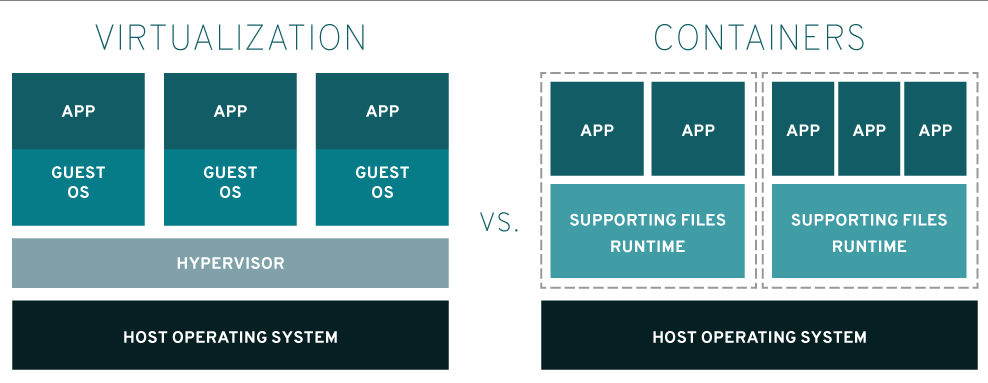
\includegraphics[scale=0.45]{Imagenes/dockervsvm1.png}
\caption{Virtualización VS Containers}
\label{dock-1}
\end{figure}

Docker, en concreto, es una plataforma que mejora el sistema LXC (proyecto de contenedores de linux) combinando este sistema con herramientas propias. Actualmente se puede ejecutar tanto en Linux como en MAC o Windows, lo que hace que cada contenedor pueda ser lanzado indistintamente de la máquina o el SO. Pero, ¿esto es del todo cierto? ¿cómo puede lanzar un contenedor de Linux en Windows o viceversa? Evidentemente, esto no es posible, en el caso de Windows, por ejemplo, la solución consiste en lanzar una maquina virtual con un kernel de Linux sobre el hyper-V (el hypervisor de windows a partir de Windows 10) o sobre una maquina virtual Virtualbox (versiones anteriores) y ejecutar todos los contenedores de Linux sobre esa máquina virtual. Sin embargo, los contenedores de Windows únicamente es posible lanzarlos desde este mismo sistema operativo \cite{Dck-10}. \par

Cada imagen del contenedor Docker se almacenan físicamente en el disco con una estructura de diferentes capas que hace que, cada imagen, sea aún más ligera de almacenar. Dicha cuestión ocurre porque se puede aplicar algo similar al concepto de herencia entre las diferentes máquinas permitiendo así, que cada imagen sea a su vez parte de la máquina de la que hereda. Para entender esto, debemos saber cuál es la estructura de un Dockerfile que define la imagen de un contenedor Docker. Cada una de estas imágenes se etiquetan con un nombre de modo que sean fáciles de manejar posteriormente.\par

Un Dockerfile es un fichero que contiene diferentes macros para compilar y crear la imagen. La primera instrucción de dicha imagen siempre es el contenedor base \cite{Dck-11}. Cada una de las instrucciones que se ejecuten da lugar a una nueva capa (layer) que se almacena y se puede compartir, si fuera necesario, entre otros contenedores. Siguiendo con el símil de los contenedores físicos, cada contenedor tiene un límite de capacidad, que en este caso es un límite de capas se pueden almacenar para un solo contenedor. Cuando se ha realizado este trabajo el límite estaba en 150 capas. \cite{Dck-12}. \par

Este diseño de capas nos permite, además de ocupar menos espacio en disco, poder tenerlas en un repositorio y solo descargarnos las capas que no tenemos. Docker nos proporciona la herramienta Docker Hub, un repositorio público similar a los repositorios de código pero que, a diferencia de estos, almacena las imágenes de los contenedores. Además, podremos descargar cualquier imagen y ejecutarla en cualquier máquina que tenga instalado Docker.\par

Por otro lado, Docker nos ofrece la herramienta “compose”. Dicha herramienta nos permite lanzar y administrar, con una sola instrucción, diversas aplicaciones y servicios de múltiples contenedores. Para ello, se define un fichero en formato YAML según la estructura definida por Docker \cite{Dck-13}. Gracias a dicha herramienta, es muy sencillo levantar y manejar toda una estructura de aplicaciones y diferentes servicios.\par

Por último, vamos a comentar por qué hemos elegido Docker frente a otras posibilidades. Aunque algunas empresas nos recomiendan subcontratar los nuevos proyectos relacionados con tecnologías de Big Data en vez de hacer un proyecto DIY (Do It Yourself) \cite{Dck-14}, dada la naturaleza de nuestro trabajo, Docker es la mejor opción. Docker nos ofrece ventajas tales como replicar y modificar las máquinas fácilmente, podemos usarlo desde cualquier máquina descargando la imagen directamente de Docker Hub y, posteriormente, poder probarlo en la nube sin tener que realizar grandes modificaciones. De esta forma, realizar cualquier cambio no requiere hacer copias de una máquina virtual entera sino modificar el Dockerfile de la máquina correspondiente. En la figura \ref{dock-2} \cite{Dck-15} podemos comprobar que el rendimiento que se obtiene con Docker es mejor que el de usar una máquina virtual KVM tanto para el arranque de las máquinas como para el benchmark UnixBench \cite{Dck-15}. En concreto, obtenemos un 30\% más de rendimiento con Docker que con KVM aunque, evidentemente, lo mejor es ejecutarlo sobre la máquina directamente. También podemos comprobar en la figura \ref{dock-3}  \cite{Dck-15} que el tiempo que tarda en arrancar una máquina Docker es de 5 segundos, mientras que una máquina virtual KVM tarda 15 segundos.\par

\begin{figure}[htp]
\centering
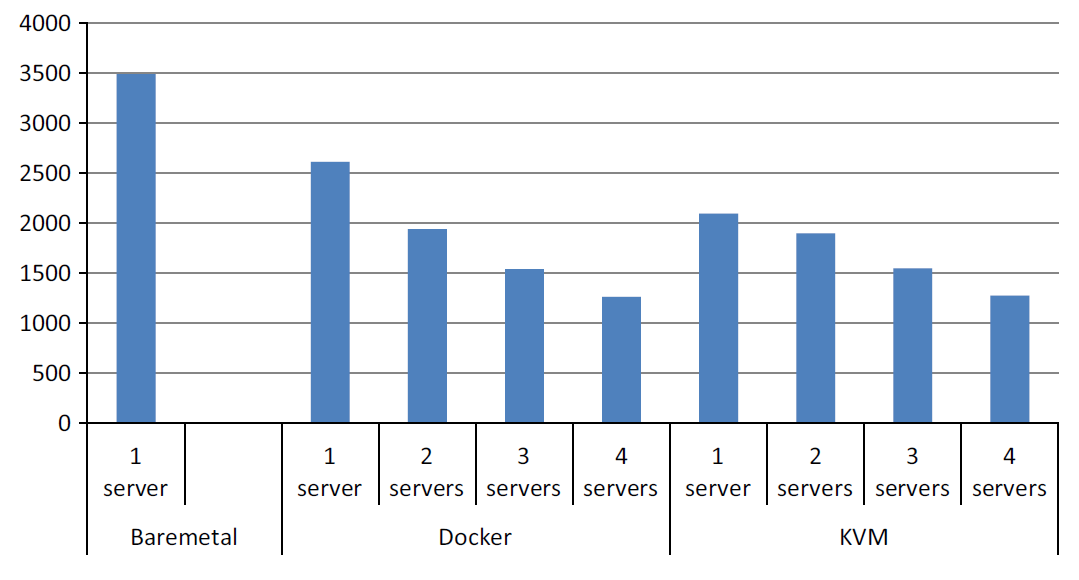
\includegraphics[scale=0.40]{Imagenes/dockervsvm2.png}
\caption{Rendimiento del benchmark con el índice UnixBench para el software sobre una máquina real, sobre Docker y sobre KVM}
\label{dock-2}
\end{figure}

\begin{figure}[htp]
\centering
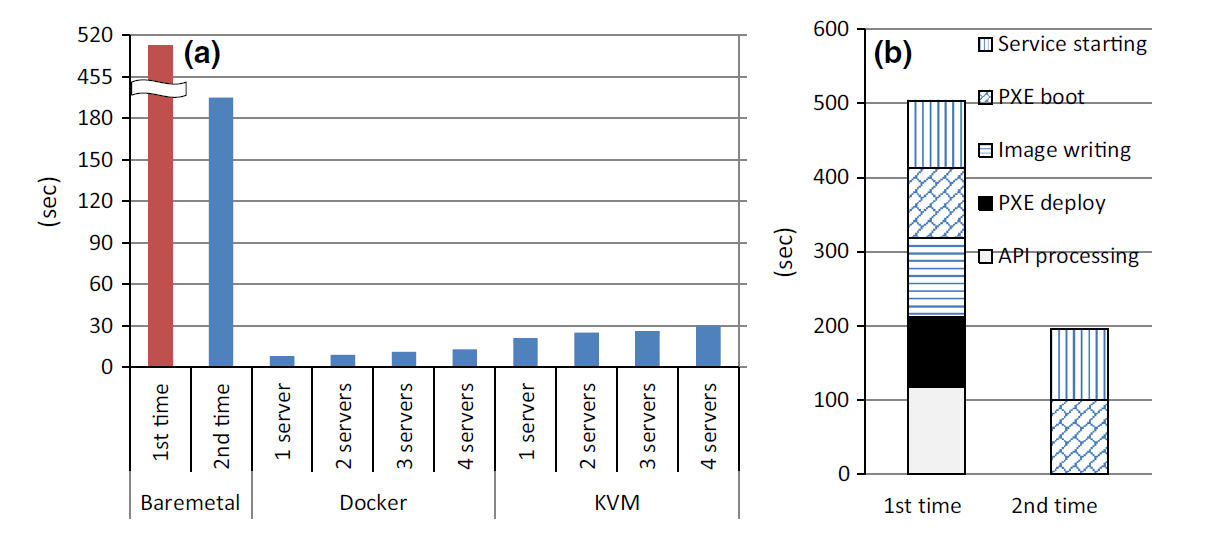
\includegraphics[scale=0.40]{Imagenes/dockervsvm3.png}
\caption{Tiempo de arranque sobre una máquina real, sobre Docker y sobre KVM}
\label{dock-3}
\end{figure}


\subsection{Apache Hadoop\label{Hadoop}}



Obviamente, cuando hablamos de Big Data tenemos que hacer referencia a Apache Hadoop. Para la realización de esta herramienta, se basaron en dos en dos artículos publicados por Google sobre su sistema de ficheros distribuido \cite{Hdp-2} y MapReduce \cite{Hdp-3}. El sistema de ficheros de Hadoop fué bautizado como HDFS convirtiéndose en una herramienta muy popular de la que hacen uso grandes empresas como Yahoo!,   Last.fm, Facebook o el New York Times. Además de esto, en 2009, Hadoop superó el récord de Google en ordenar un terabyte de datos en menos tiempo \cite{Hdp-1}. Además de esto, Apache Hadoop forma parte de Apache Foundation, lo que quiere decir que es totalmente OpenSource.\par

Actualmente, la arquitectura de la versión 3 de Hadoop, está formada por cuatro módulos principales y sus diferentes servicios \cite{Hdp-4}:\par

\begin{itemize}
	\item \textbf{Hadoop Common}: Este paquete contiene las utilidades comunes que soportan todos los demás módulos de Hadoop.
	\item \textbf{Hadoop Distributed File System (HDFS)}: Es el sistema de ficheros distribuido de Hadoop. Por definición es un sistema de ficheros distribuidos que proporciona un alto rendimiento a los datos de aplicación. Tiene una estructura maestro/esclavo que se compone de los siguientes servicios:
	\begin{itemize}
		\item \textbf{Namenode}: Administra el espacio de nombres del sistema de ficheros y regula el acceso a los diferentes ficheros. Además, asigna el datanode donde se almacenará cada bloque físico de cada fichero para que quede balanceado dicho sistema. Por tanto, en este nodo se encontrarán los metadatos de donde se encuentra cada bloque.
		\item \textbf{Datanode}: Es un nodo de almacenamiento. En dicho nodo existirán bloques de datos, asignados por el NameNode.
		\item \textbf{Secondary NameNode}: Es una réplica del namenode que se usa como copia por si en algún momento el NameNode cae. Se hace una copia de los metadatos cada hora o cada millón de transacciones por defecto.
		\item \textbf{Checkpoint node}: Al igual que el Secundary NameNode, hace copias de seguridad del NameNode, pero no tiene la capacidad de sustituirlo.
	\end{itemize}
	\item \textbf{Hadoop YARN}: Este módulo es el framework que gestiona los trabajos y los diferentes recursos del cluster. La idea consiste en separar la planificación y la supervisión de los diferentes trabajos sobre Hadoop. También usa una estructura de maestro/esclavo para los cuales se suministran los siguientes servicios:
	\begin{itemize}
		\item \textbf{Resource Manager}: Este servicio se considera el “maestro”. Tiene dos funcionalidades principales, la función de Scheduler (planificador) y la función de ApplicationsManager (gestor de aplicaciones). Como planificador debe ser capaz de asignar los recursos necesarios a cada aplicación cuando lo necesite o reiniciar una aplicación en caso de fallo. Como gestor de aplicaciones es el encargado de asignar trabajo a cada uno de los componentes del cluster.
		\item \textbf{Node Manager}:Es el responsable de iniciar y administrar los trabajos para una nodo del cluster.
		\item \textbf{ProxyServer}: Por defecto, se ejecuta junto al Resource Manager, pero se puede ejecutar por separado. Se encarga de reducir ataques web que puedan producirse a través de YARN.
	\end{itemize}
	\item \textbf{Hadoop MapReduce}: Es el módulo para el procesamiento paralelo de grandes conjuntos de datos. Este sistema está basado en YARN. Además, tiene un servicio adicional que podemos añadir: 
	\begin{itemize}
		\item \textbf{HistoryServer}: simplemente muestra a través de una web los logs que producen los diferentes trabajos de MapReduce.
	\end{itemize}
\end{itemize}

HDFS, como ya hemos dicho, es el sistema de ficheros de Hadoop, cuya característica más importante es que es distribuido, aunque no es la única característica que posee. HDFS, como los sistemas de ficheros convencionales, distribuye los diferentes ficheros en bloques de un tamaño fijo, normalmente de 128 MB, ya que suponen ficheros de gran tamaño, aunque esto es modificable. Dichos bloques están divididos entre los diferentes nodos del cluster de forma que sea más fácil realizar diversos tratamientos sobre ellos de forma paralela. Además de esto, contamos con la replicación de los distintos bloques, según establezcamos cuantas replicaciones de bloque queramos. Esto tiene muchas implicaciones tales como cuando cae uno de los nodos, siempre tenemos los datos disponibles en otro nodo, si uno de los nodos cae o se rompe el disco duro, podemos volver a generar dicho nodo a partir de los metadatos del namenode y la replicación de bloques. Dicho esto, podemos ver que no tiene sentido montar un RAID sobre el servidor, ya que el sistema de Hadoop te proporciona dicha funcionalidad.\par

MapReduce consiste en uno o varios procesos distribuidos que manejan grandes volúmenes de datos. Tiene dos funciones principales, map y reduce. La función Map genera una tupla clave/valor intermedios y la función Reduce combina esos valores para cada clave para obtener un resultado. Dicho esto, se muestra en la figura \ref{hdImg1} \cite{Hdp-1} un ejemplo de cómo funcionaria gráficamente:\par

\begin{figure}[htp]
\centering
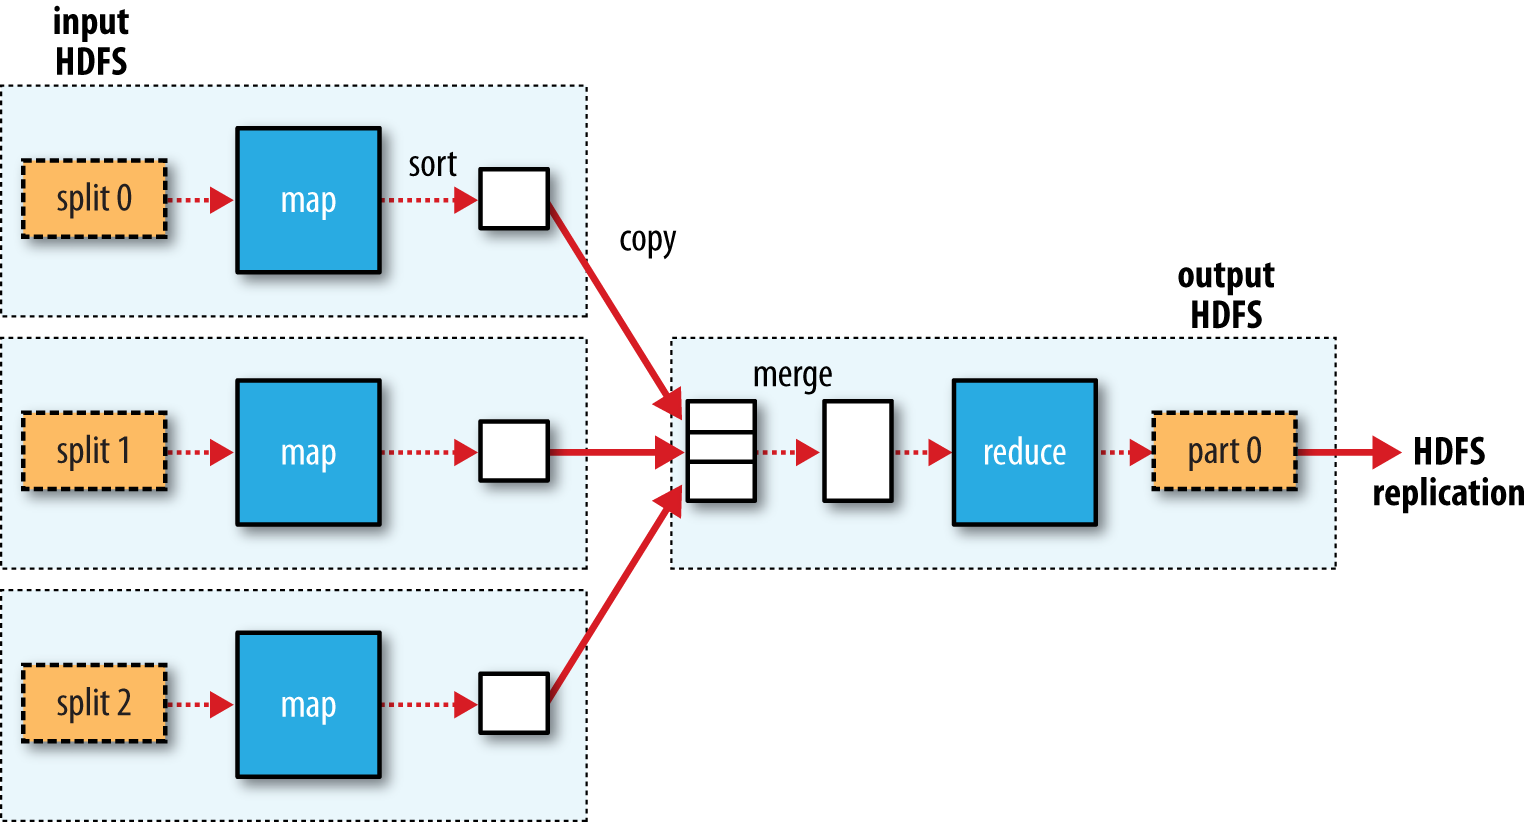
\includegraphics[scale=0.28]{Imagenes/hadoop1.png}
\caption{Funcionamiento de Map Reduce sobre HDFS. }
\label{hdImg1}
\end{figure}

Por último, decir que Apache Hadoop está programado en Java y necesitamos la JVM (Java Virtual Machine) para ejecutarlo.\par


\subsection{Apache Spark\label{Spark}}

Apache Spark surge de las problemáticas de usar Hadoop en plataformas generales, específicamente cuando hablamos de algoritmos de aprendizaje automático en las que se necesitaban realizar múltiples iteraciones sobre los mismos datos. El equipo de Spark diseñó un API basada en la programación funcional, en concreto usaron el lenguaje Scala que permitía, en un solo trabajo, realizar varias interacciones de MapReduce \cite{Spk-1}. Apache Spark lanzó la versión 1.0 en 2014 y Spark 2.0 en 2016, realizando regularmente nuevas aportaciones al proyecto \cite{Spk-2}.Actualmente está disponible la versión 2.3, que usaremos en este trabajo. A continuación hablaremos de los aspecto s más importantes de este framework.\par

Una de las características más importantes de cómo funciona Spark es como distribuye el trabajo. Spark soporta un flujo de datos acíclico creando un \textbf{DAG} (Directed Acyclic Graph) de etapas de trabajo que, por definición del mismo, es un grafo de trabajo sin ciclos \cite{Spk-5}. Esto nos permitirá repartir las tareas de trabajo entre los distintos nodos del cluster y favorecer la recursión dentro del mismo. Para poder añadir trabajos a este DAG podemos hacerlo a través de la variable Spark Context. Cuando añadimos un trabajo al Spark Context, Spark reorganiza el DAG y optimiza la gestión de las tareas añadidas. Por otro lado, la siguiente característica más importante de Spark son los \textbf{RDD} (Resilient Distributed Dataset) que consiste en una colección inmutable de datos particionada con la que se puede operar de forma paralela. Sobre estos RDD podemos realizar diferentes operaciones como MapReduce o cualquiera que nos permitan los módulos de Spark \cite{Spk-4}.\par

En cuanto a la arquitectura de un cluster de Spark, tenemos dos tipos de nodos principales. El más importante es el \textbf{nodo master}, que es el que coordina a los demás nodos. Este nodo dirige a los \textbf{nodos esclavos} (o slaves) que son los que ejecutan los trabajos de Spark. Además de estos nodos, podemos añadir un servicio de monitorización de trabajos que se llama \textbf{history-server}. Finalmente, como se ha explicado, podemos ver cómo se comunican y distribuyen los trabajos en la figura \ref{SpkImg-1} \cite{Spk-6}.Aunque tengamos esta estructura, también podremos integrar Spark con un cluster de Hadoop sin realizar grandes modificaciones. Para integrar el cluster simplemente tendremos que añadir las librerías de spark al HDFS y lanzar los trabajos desde un nodo que contenga Spark, esto hace que Spark esté siendo tan famoso ya que puedes reutilizar la estructura si existiera manteniendo ambos framework.\par

\begin{figure}[htp]
\centering
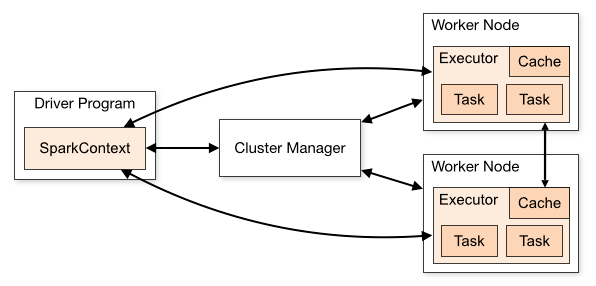
\includegraphics[scale=0.65]{Imagenes/spark1.png}
\caption{Comunicación en los nodos de Apache Spark para la realización de trabajos}
\label{SpkImg-1}
\end{figure}

Por último, Spark se divide entre diferentes módulos que nos facilitará diferentes operaciones sobre los datos  \cite{Spk-3}:\par

\begin{itemize}
	\item \textbf{Spark Core Engine}: Es el módulo principal de Spark. Sobre este módulo se ejecutan todos los demás. Permite la persistencia en memoria de forma que permita una gran velocidad al pedir datos.\par
	\item \textbf{Spark Sql y DataFrames}: Este módulo nos permite trabajar con datos estructurados con Spark. Sobre estos datos podemos realizar consultas SQL.\par
	\item \textbf{Spark Streaming}: Este módulo nos permite trabajar con microbaching, creando aplicaciones escalables y tolerantes a fallos.
	\item \textbf{MLlib}: Este módulo es el que contiene los diferentes algoritmos de aprendizaje automático que podemos usar con Spark.
	\item \textbf{GraphX}: Este módulo nos permitirá realizar procesamiento de gráficos en paralelo. En definitiva, con este módulo, tenemos una serie de operaciones sobre grafos que nos permite manejar los mismos de una forma rápida y escalable.
	\item \textbf{SparkR}: Este módulo proporciona una interfaz ligera de R que implementa las diferentes operaciones distribuidas que se aplican sobre los RDDs de Spark.
\end{itemize}

A partir de aquí podemos ver toda la funcionalidad que nos aporta Spark frente a Hadoop \cite{Spk-7}. Por otro lado, al igual que con Hadoop, tenemos varios lenguajes con los que programar los diferentes trabajos. En nuestro caso usaremos Python, pero podríamos usar R o Java. También podríamos usar otros lenguajes como C\# a partir de diferentes módulos que están a disposición en la página oficial de Spark \cite{Spk-6}.\par


\subsection{Apache Kafka\label{Kafka}}

Apache Kafka surgió de la empresa Linkedin a partir del sistema que tenían para recopilar múltiples métricas de sus sistemas y aplicaciones. Tenían un sistema que registraba la información de la actividad de cada usuario a partir de diferentes XMLs con una cantidad indefinida de variables, lo que lo hacía complejo y propenso a fallos. Para solucionar estas problemas se realizaron diferentes estudios que llevaron a Linkedin a usar una aplicación de gestión de mensajes, en concreto ActiveMQ. Cuando comenzaron a usar ActiveMQ descubrieron que tenían una serie de necesidades adicionales que dicho software no contemplaba. La imposibilidad de escalar dicho software y una serie de fallos que descubrieron posteriormente cuando estaban procesando sus datos, dio lugar a que Linkedin realizará un desarrollo propio. Dicho desarrollo fue bautizado como Kafka. Kafka debía reunir una serie de características para solventar los problemas concretos de Linkedin que con un sistema de gestión de mensajes tradicional no bastaba. Necesitaban que tanto los productores como los consumidores de los mensajes pudieran estar desacoplados a la hora de insertar u obtener un mensaje. También necesitaban que los mensajes fueran persistentes en las colas de mensajes de forma que los múltiples consumidores pudieran hacer uso de los mensajes. A su vez, era necesario optimizar al máximo el tiempo que se necesitaba en procesar los mensajes. Por último, era importante que pudieran escalar el sistema horizontalmente si es necesario por la cantidad de mensajes o por nuevos tipos de mensajes. Finalmente, hemos de subrayar que Kafka está escrito en el lenguaje Scala y se lanzó como proyecto Open Source y forma parte de la Apache Software Foundation \cite{Kfk-1}. 
Para entender Kafka, debemos de tener en cuenta que es una simple cola de mensajes en la que varios productores y consumidores pueden estar a la vez enviando y recibiendo mensajes. Los mensajes de Kafka son persistentes, esto hace que se pueda ver como el gran fichero de log de varias aplicaciones y que, posteriormente, otras aplicaciones leen para aplicar a esos datos diferentes procesos convirtiéndolos, por ejemplo, en estadísticas \cite{Kfk-6}. La persistencia de estos mensajes se mide a través de una determinada métrica de tiempo o de espacio y es lo que permite tener varios tipos de consumidores. En el caso de una arquitectura Lambda, por ejemplo, podemos leer de la misma cola tanto para la bach layer como para la bach layer y esto quiere decir que la toda la información de que proviene de una cola se mantiene en un mismo sistema sin necesidad de replicar datos.Además, otra de las características más importantes de Kafka, es que podemos instalarlo como un sistema distribuido lo que lo hace muy tolerante a fallos.\par

Podemos diferenciar Kafka en las siguientes partes:\par

\textbf{Mensajes y lotes (batch)}: La forma en que se introduce y se saca la información en Kafka es a través de mensajes. Cada mensaje, para Kafka, es una serie de bytes sin significado alguno a excepción de la parte de metadatos que contienen una clave y una marca de tiempo. La clave se puede usar para distribuir los datos en diferentes particiones o para hacer un seguimiento de los mensajes. Los mensajes se pueden escribir en lotes (batch), que no es otra cosa que una colección de mensajes. Eso nos permite escribir y obtener los mensajes mucho más rápido, ya que podemos escribir o recibir varios mensajes en una sola petición. Los mensajes se mantienen persistentes hasta un tiempo definido o hasta que la cola llegue a una cantidad fija de espacio, por ejemplo, 20 GB. Si se llega al límite por espacio, se borrarán los primeros mensajes que llegaron a la cola, y si llega al límite por tiempo se borrarán cuando haya pasado el tiempo de caducidad del mensaje.\par

\textbf{Estructuras}: Aunque para Kafka los mensajes son únicamente bytes, se recomienda usar algún tipo de estructura. Esto no es una propiedad de Kafka como tal, pero es una recomendación muy útil. Las estructuras más utilizadas sobre los mensajes de Kafka son JSON y XML.\par

\textbf{Topics y particiones}: Al igual que en una base de datos tenemos tablas o en un sistema de ficheros tenemos directorio, Kafka organiza los mensajes por topics. Estos topics, a su vez, se dividen en particiones donde se almacenan los mensajes. Los mensajes se almacenan en orden de llegada y cada partición puede estar en diferentes servidores. Además. puede haber replicación en las particiones o no, según las necesidades. En la figura \ref{Kfk-img-1} \cite{Kfk-2} podemos ver cómo se escriben los mensajes de un topic en diferentes particiones. Además, a través de las claves de los mensajes, podemos repartir los mismos entre las diferentes particiones.\par


\begin{figure}[htp]
\centering
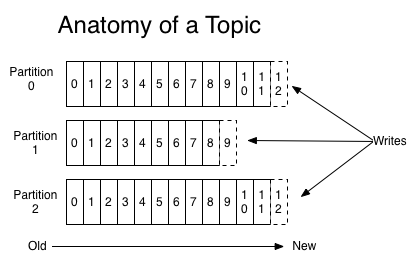
\includegraphics[scale=0.75]{Imagenes/kafka1.png}
\caption{Funcionamiento del Topic en Kafka con sus particiones}
\label{Kfk-img-1}
\end{figure}

\textbf{Productores y consumidores}: Para Kafka, sus clientes, son los diferentes usuarios del sistema que escriben o leen la información, es decir, los productores y los consumidores. Los productores o publicadores son los encargados de escribir los mensajes en un topic. Sin embargo, les da lo mismo en qué partición se encuentre cada mensaje, por lo que será Kafka el encargado de distribuir los mensajes en las diferentes particiones. Opcionalmente los productores pueden añadir una clave al mensaje y así poder repartir ellos mismos los mensajes entre las diferentes particiones. A la misma vez, pueden haber varios productores escribiendo en un mismo Topic. Los consumidores o lectores son los encargados de leer y consumir el mensaje, con la característica de que el mensaje no se borrará una vez leído si no, como hemos dicho, según la caducidad del mismo. Cada uno de los consumidores se suscribe a un tema he irá leyendo los mensajes en el orden en el que se han producido. Además, puede haber varios consumidores leyendo de un mismo topic y de una misma partición. Los consumidores pueden leer desde el principio de la cola o empezar con un desplazamiento u offset específico. Una vez vaya leyendo los mensajes, el consumidor sabrá por cuál se ha quedado y podrá seguir leyendo a partir del siguiente mensaje. Esto significa que los consumidores pueden detenerse o reiniciarse y sabrán volver al punto por donde se habían quedado. También existen grupos de consumidores que leen cada uno una parte de la cola, de forma que pueden ir procesando cada uno una parte del tema. Estos grupos de consumidores también son tolerantes a fallos ya que, si alguno deja de consumir automáticamente, los demás se irán equilibrando para que no se pierdan mensajes. Por último decir que, a un consumidor de un grupo se le puede asignar una partición de forma que sea a ese consumidor el que lee, mayormente, dicha partición. Decimos mayormente porque si hay un fallo por parte de otro consumidor, para que una partición no se quede sin leer, automáticamente se le asignará mensajes de otras particiones para que los procese. Podemos ver como un grupo de consumidores consumen un topic en la figura \ref{Kfk-img-2} \cite{Kfk-1}.

\begin{figure}[htp]
\centering
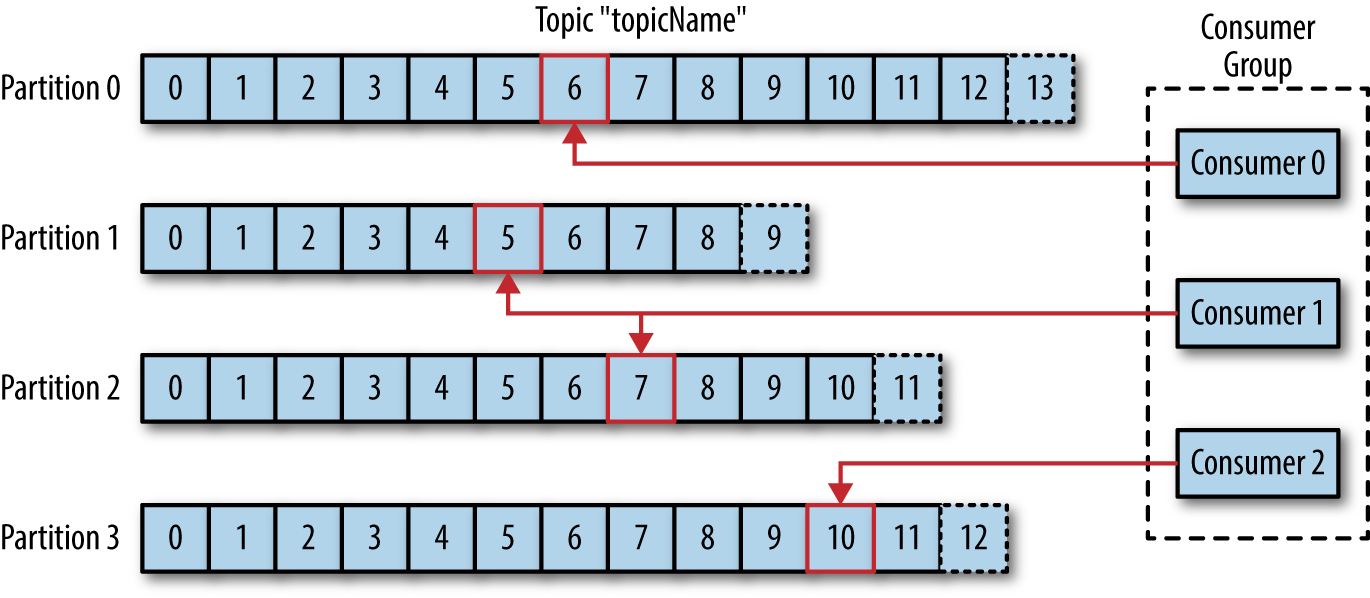
\includegraphics[scale=0.30]{Imagenes/kafka2.png}
\caption{Distribución del trabajo entre consumidores de un Topic Kafka}
\label{Kfk-img-2}
\end{figure}

\textbf{Brokers y Clusters}: Cada servidor con Kafka se le llama broker y es el encargado de recibir y enviar los mensajes desde los productores a los consumidores. Como ya sabemos, una vez recibe un mensaje, estos deben permanecer en disco, esto lo hace el broker asignándole el offset correspondiente y eliminando los mensajes que han caducado. El broker también es el encargado de gestionar las diferentes particiones siendo capaz de manejar miles de particiones y millones de mensajes, dependiendo del hardware donde resida. Un broker está diseñado para formar parte de un cluster junto a más brokers, los cuales son gestionados a través de Zookeeper. Mediante este mismo, se gestiona quién será el líder del cluster, encargado de repartir las particiones, controlar la replicación de datos y revisar fallos. Si el líder falla, será Zookeeper el encargado de asignar un nuevo líder. 


\subsection{Elastic\label{Elastic}}

Elasticsearch es un motor de búsqueda y recuperación de documentos de código abierto construido sobre Apache Lucene. En torno a este motor se ha formado la empresa Elastic que promociona Elasticsearch junto a su stack de tecnologías aportando a diferentes empresas un sistema de búsqueda en tiempo real avanzado y versátil \cite{Elk-1}.\par

Actualmente podemos definir Elasticsearch como un motor de búsqueda y análisis de texto, con una interfaz RESTful, compatible con múltiples usuarios y capaz de almacenar grandes cantidades de datos. Junto con este motor encontramos Elastic Stack, una serie de tecnologías que permiten conectarte a Elasticsearch de una forma más segura y sencilla, tanto para escribir como para leer datos.\par

Elastic Stack tiene como núcleo Elasticsearch y está formado por Kibana, Logstash, Beats, ECE y X-Pack. Cada uno de estos módulos son totalmente independientes e interoperables unos con otros. A continuación, explicamos cada uno de ellos \cite{Elk-4}:
\begin{itemize}
	\item \textbf{Elasticsearch}: Considerado el corazón de Elastic Stack, se trata del motor de búsquedas basado en Apache Lucene. Puedes insertar documentos de tipo JSON y hacer analiticas o busquedas sobre ellos. Para realizar las inserciones, las modificaciones y las consultas hay que usar una API RESTful con diferentes operaciones tipo GET, PUSH, PUT o DELETE, acompañadas de un JSON con las operaciones a realizar. Los documentos en Elasticsearch se introducen en un índice, con un tipo y un identificador para facilitar la búsqueda y reconocer más fácilmente los distintos campos del documento. Otra característica importante es que, aunque definas un tipo en Elasticsearch, siempre puedes añadir un documento con otros campos. Finalmente, para acceder al documento podemos hacerlo desde cualquier navegador realizando las consultas de la siguiente forma: servidorElasticsearch:PORT/indice/tipo/identificador y nos devolverá el objeto JSON que pedimos.
	\item \textbf{Beats}: Este módulo puede enviar datos de diferentes fuentes, principalmente de ficheros, aunque también puede leer de bases de datos o de las propias métricas que te aporta el sistema operativo Estos datos son enviados a Logstash o a Elasticsearch sin ningún tipo de procesado previo. Se define como un agente y está escrito en Go.
	\item \textbf{Logstash}: Se trata de un sistema de procesamiento distribuido el cual obtiene datos de diferentes fuentes para insertarlos en otras, normalmente en Elasticsearch. Cuando hablamos de Logstash hablamos de un servicio con una o varias pipelines (tuberías). Cada pipeline tiene tres fases. La primera obtendrá los datos de cualquier tipo de fuente (entrada), la segunda filtra y procesa los datos y la tercera inserta los datos en Elasticsearch o cualquier otra salida.
	\item \textbf{Kibana}: Se trata de un componente que se conecta directamente con Elasticsearch que te permite manejar y visualizar la información. Te permite establecer diferentes métricas en tiempo real e ir explorando los diferentes datos que se van insertando en Elasticsearch. Además de crear diferentes gráficas también permite crear Dashboards. Para acceder a Kibana se debe hacer vía web donde podrás manejar y administrar el componente.
	\item \textbf{ECE (Elastic Cloud Enterprise)}: Sirve para administrar tanto Kibana como Elasticsearch desde un mismo punto. Gracias a este módulo podemos monitorear y administrar un cloud de Elastic Stack desde un solo punto vía web o vía consola. También tiene una modalidad en la cual puedes montar directamente Elastic sobre un servidor de Azure o AWS.
	\item \textbf{X-Pack}: Realmente esto no es un módulo como tal, sino una serie de features. Simplemente se trata de todos los componentes extras que están bajo licencia y son de pago. X-Pack se compone de:
\begin{itemize}
	\item \textbf{Security}: Nos permite tener active directory, LDAP o bien, mantener la información cifrada en Elasticsearch. 
	\item \textbf{Alerting}: Nos permite recuperar información de Elasticsearch y poner alertas como que salte la alerta cuando se suma determinado valor de una variable en un mes. Las alertas se pueden transmitir por diferentes medios como por slack o email.
	\item \textbf{Monitoring}: Nos permite ver el estado del cluster.
	\item \textbf{Reporting}: Nos permite crear Reports a través de Kibana.
	\item \textbf{Graph}: Nos permite ver diferentes conexiones entre los documentos de una forma gráfica.
	\item \textbf{Machine Learning}: Nos permite ejecutar diferentes algoritmos de machine learning sobre Elasticsearch.
	\item\textbf{ Elasticsearch SQL}: Nos permite hacer consultas sobre Elasticsearch con una sintaxis SQL.
\end{itemize}
\end{itemize}
Sobre cualquiera de los módulos se pueden instalar diferentes plugins o librerías para añadir seguridad, conectores, operaciones o incluso gráficos. Esta es una de las razones por la que Elastic Stack es tan popular ya que, al ser código libre, todo el mundo puede aportar su granito de arena, mejorar las herramientas o crear nuevos plugins. Actualmente, estamos en la versión 6.

\subsection{MongoDB\label{MongoDB}}
